\section{Results}
\label{sec:results}
\sciwms{} currently supports contour and filled-contour plots for
scalar and vector and barb plots for vector valued attributes
regardless of data topology. Figure~\ref{fig:adcirc_comp} shows a web
portal utilizing the \sciwms{} backend to compare ADCIRC model output
for Hurricane Ike with water levels observed by NOAA stations. Ongoing
development is in progress for \sciwms{} to support emerging
geophysical datasets such as ensemble model output and to provide
clear visual support for the assessment and quantification of model
skill and performance metrics.

A custom web portal was implemented for the \comt{} \ioos{} to provide researchers an intuitive interface for generating visualizations of observational and modeling data. 

\begin{figure}[ht!]
  \centering
  \begin{subfigure}[t]{0.45\textwidth}
    \centering
    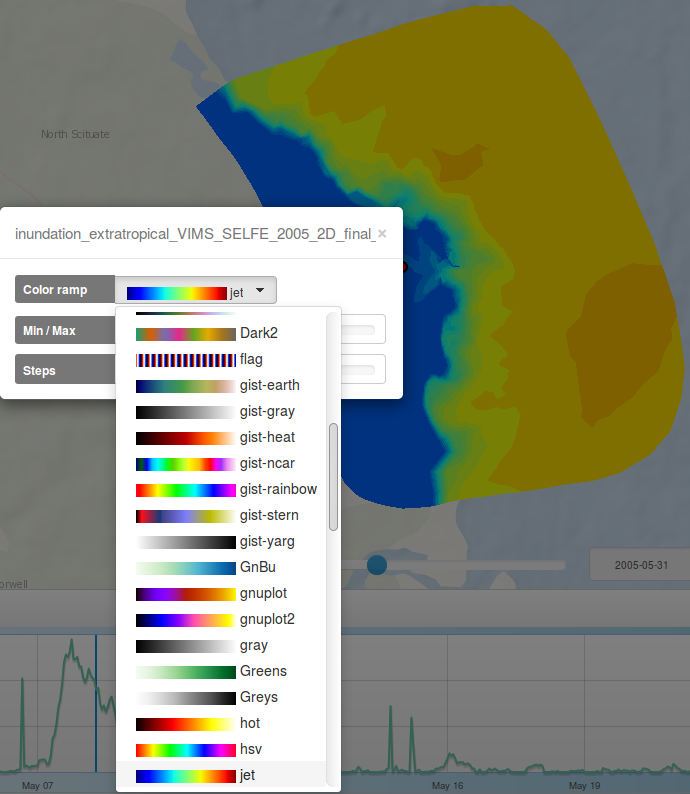
\includegraphics[height=2in]{../figs/inundation_extratropical_VIMS_SELFE_2005_final_run_waves_UI_scalar}
    \caption{Colormaps available for scalar attributes.}
  \end{subfigure}
  \begin{subfigure}[t]{0.45\textwidth}
    \centering
    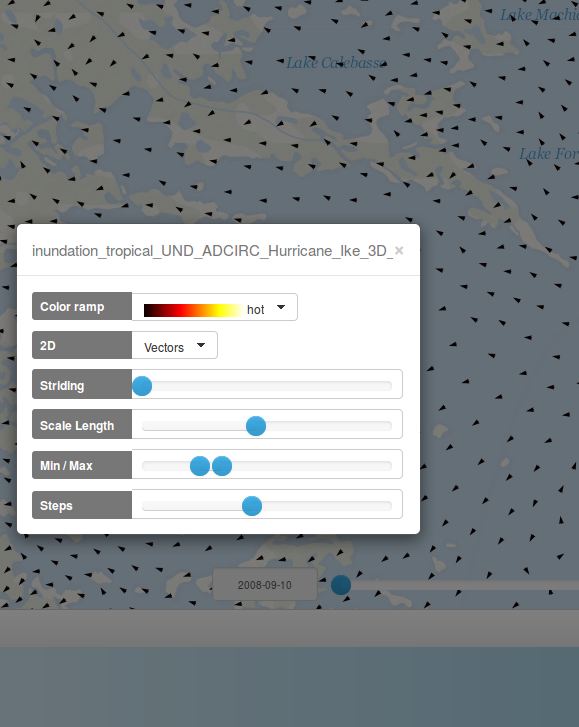
\includegraphics[height=2in]{../figs/ui_vectors_crop_inundation_tropical_UND_ADCIRC_Hurricane_Ike_3d_final_run_with_waves}
    \caption{Parameters for visualizing vector fields.}
  \end{subfigure}
  \caption{User interface for manipulating rendering style parameters
    to be sent to \sciwms{} via HTTP. The images behind the UI
    controls are the rendering returned by \sciwms{}.}
\end{figure}

\begin{figure}[ht!]
  \centering
  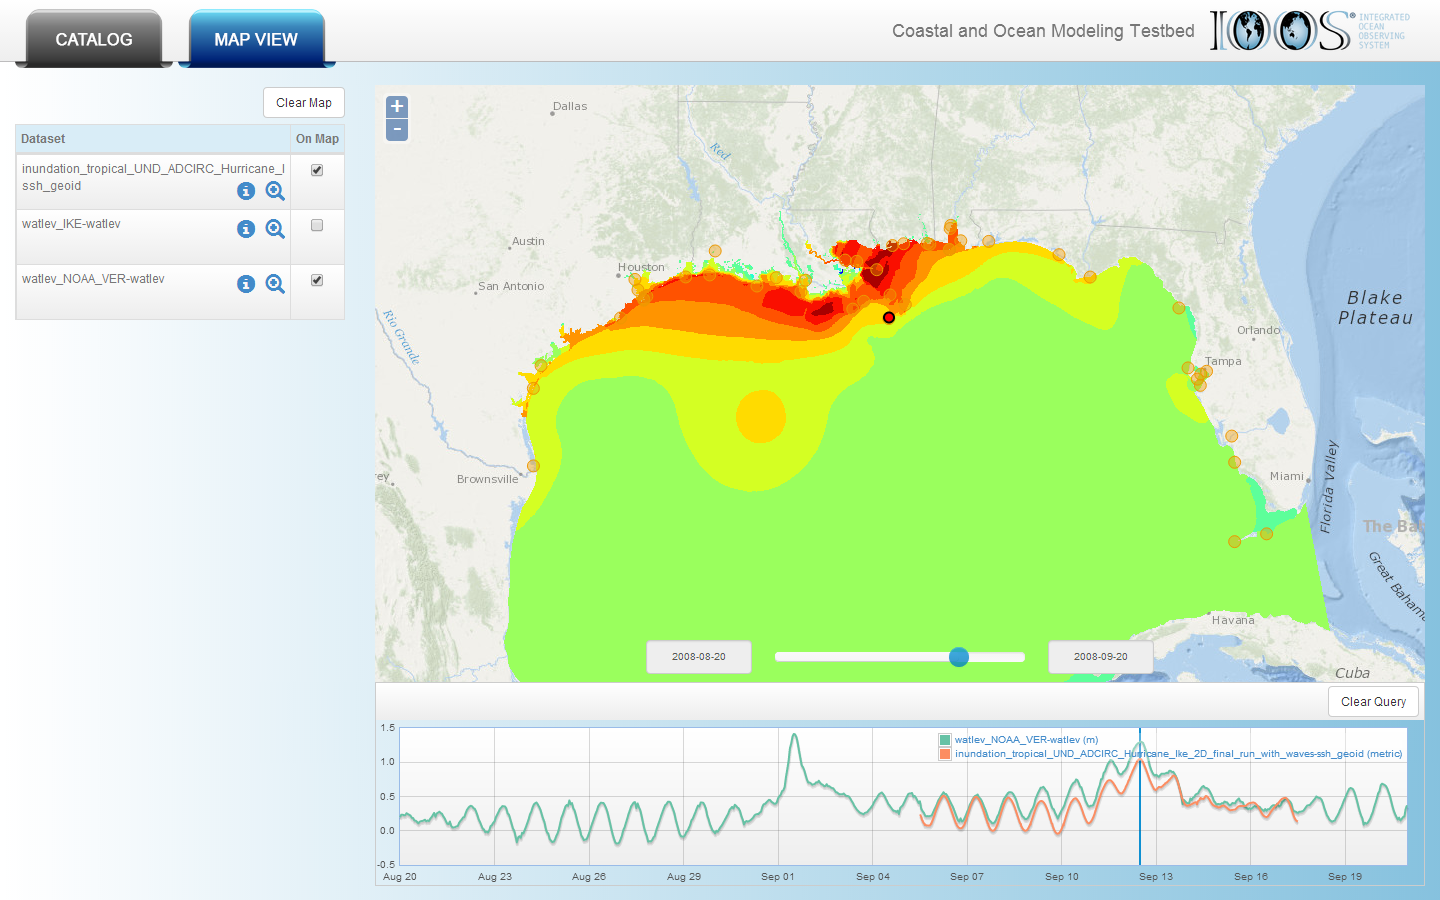
\includegraphics[width=\columnwidth]{../figs/SciWMS_ModelObsComparison}
  \caption{Comparison of ADCIRC (unstructured topology) model results
    with observed water levels in the Northern Gulf of Mexico for
    Hurricane Ike. Verified observed water levels are from NOAA's
    Station 8760922 (red dot on map). The map shows modeled water
    levels (in meters above the geoid) at the peak of the storm in
    southern Louisiana. The time series plot shows both the modeled
    (green) and observed (orange) water levels. The vertical blue line
    in the time series plot corresponds to the current time of the
    map.}
  \label{fig:adcirc_comp}
\end{figure}

\begin{figure}[ht!]
  \begin{subfigure}[t]{0.45\textwidth}
    \centering
    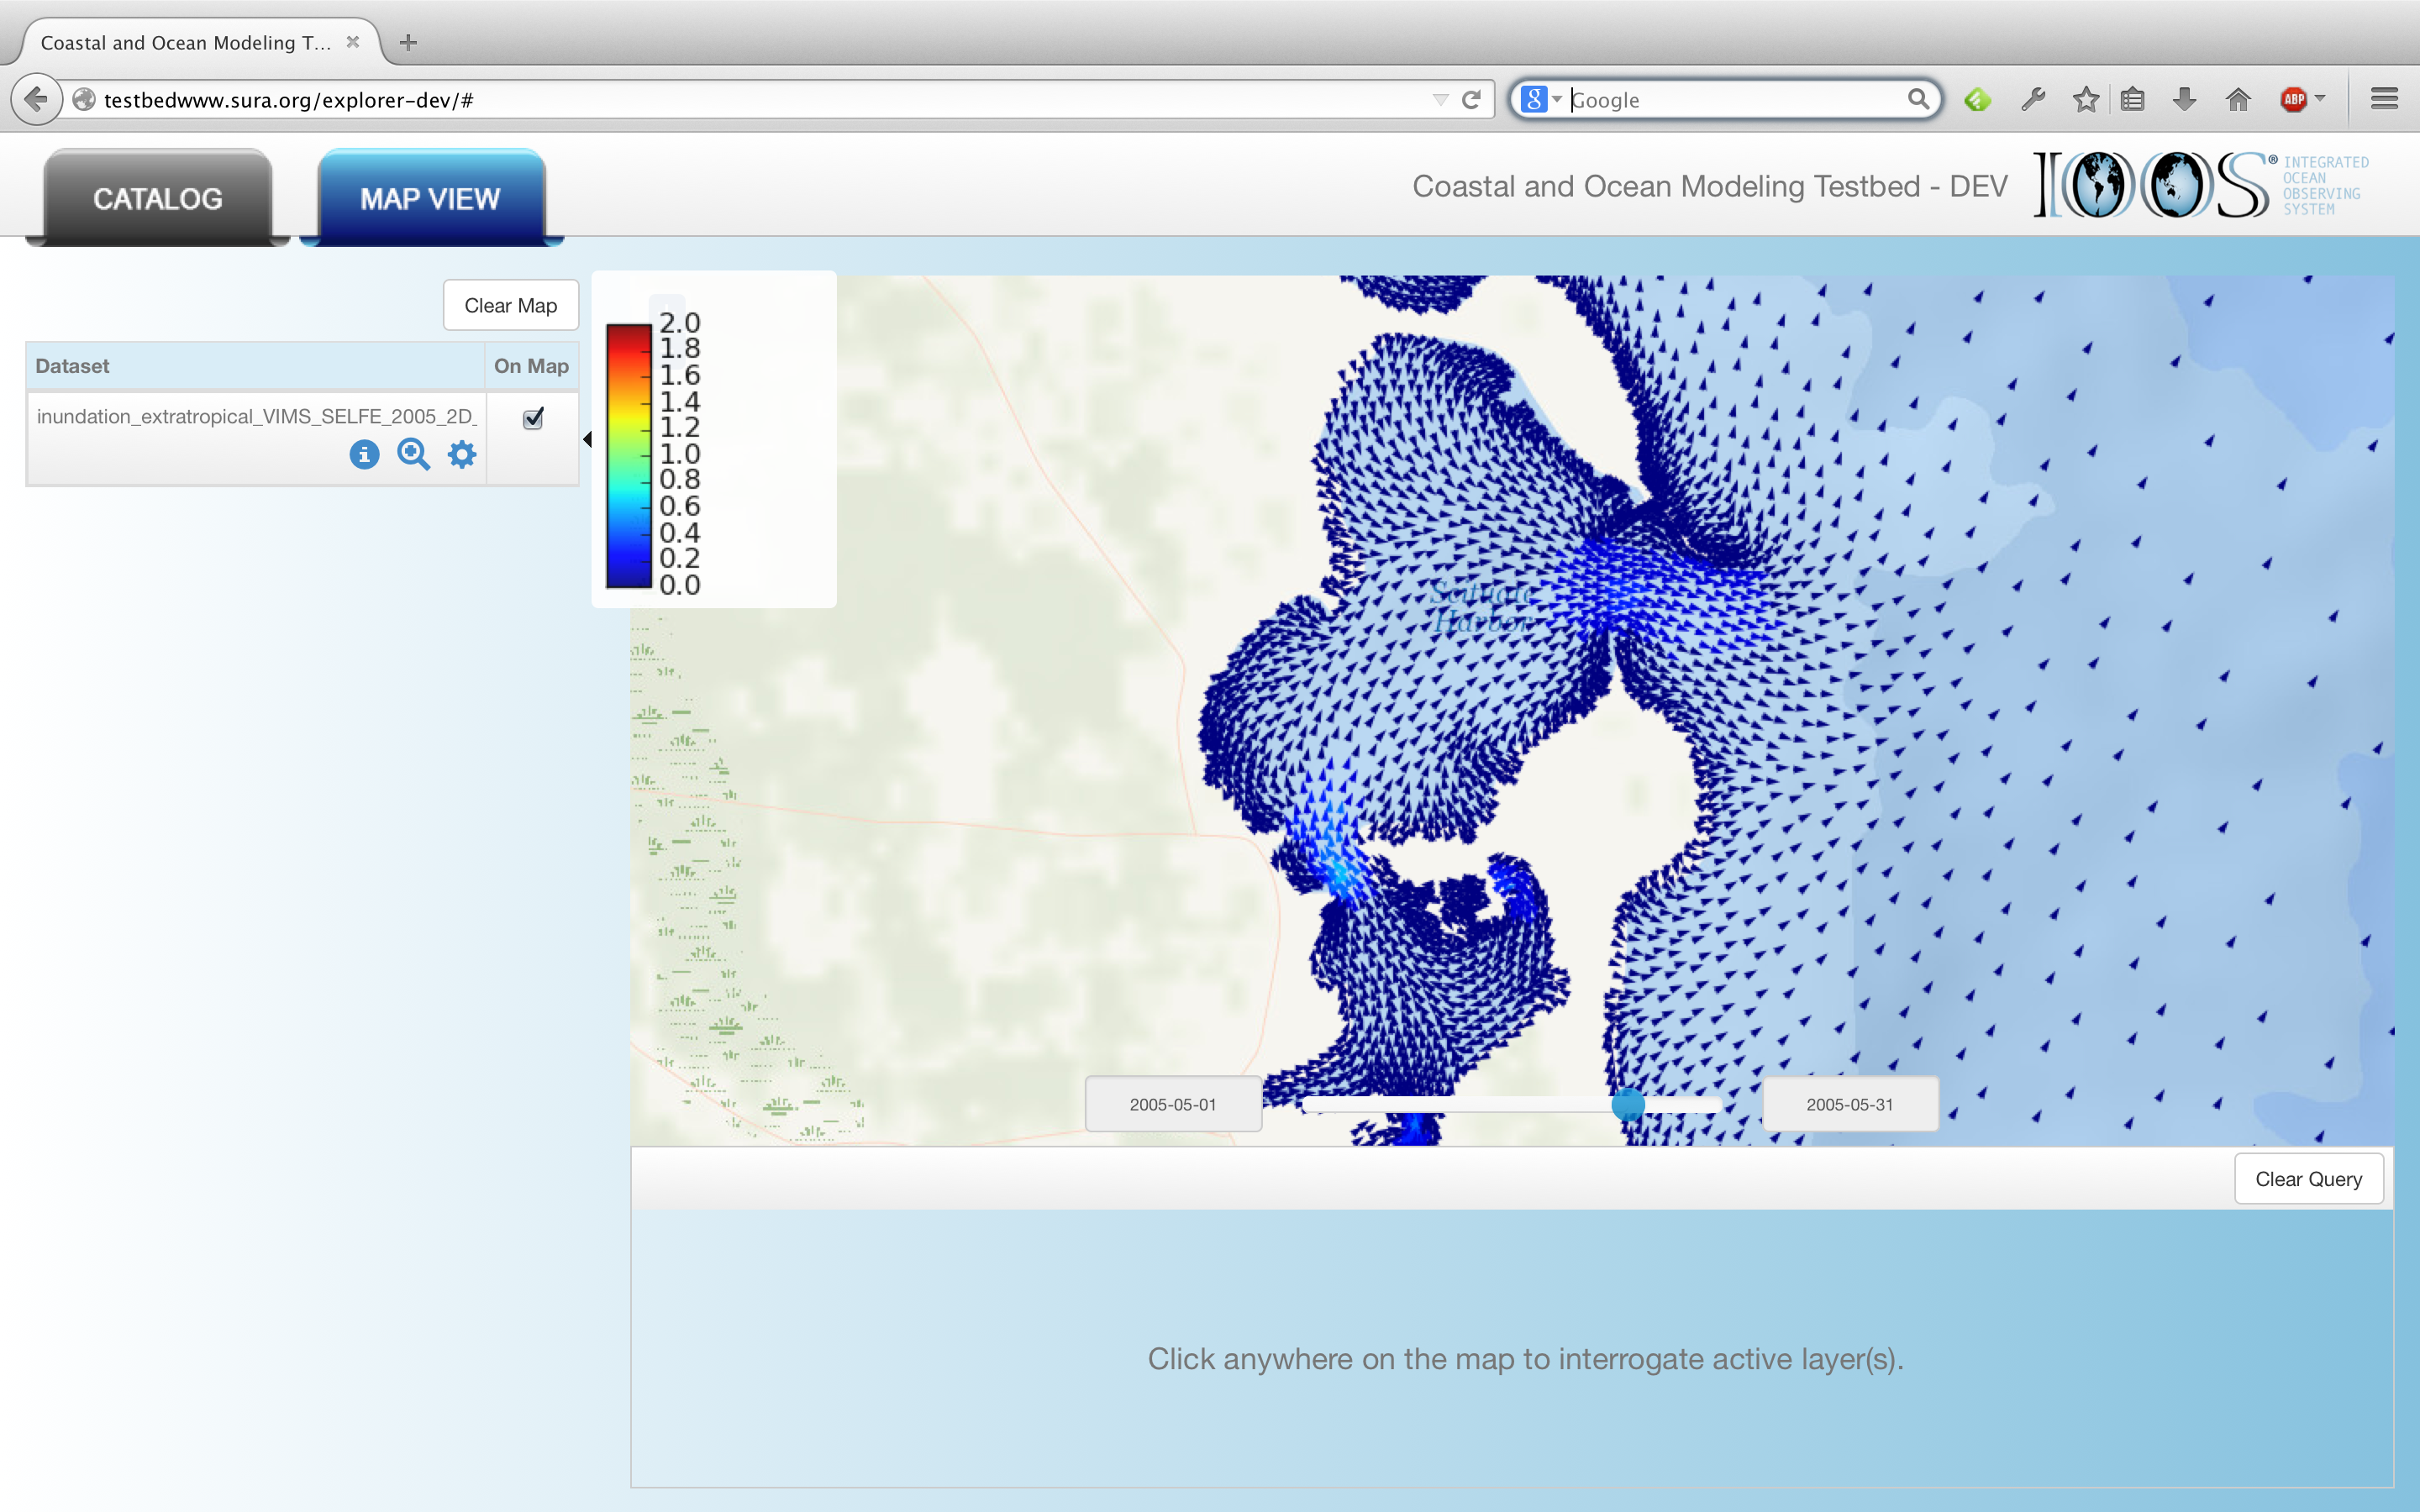
\includegraphics[width=\columnwidth]{../figs/vims_selfe_ubaratropic_vbaratropic_chesapeake_bay}
    \caption{SELFE model of current
      direction and speed in the Chesapeake Bay area.}
  \end{subfigure}
  \begin{subfigure}[t]{0.45\textwidth}
    \centering
    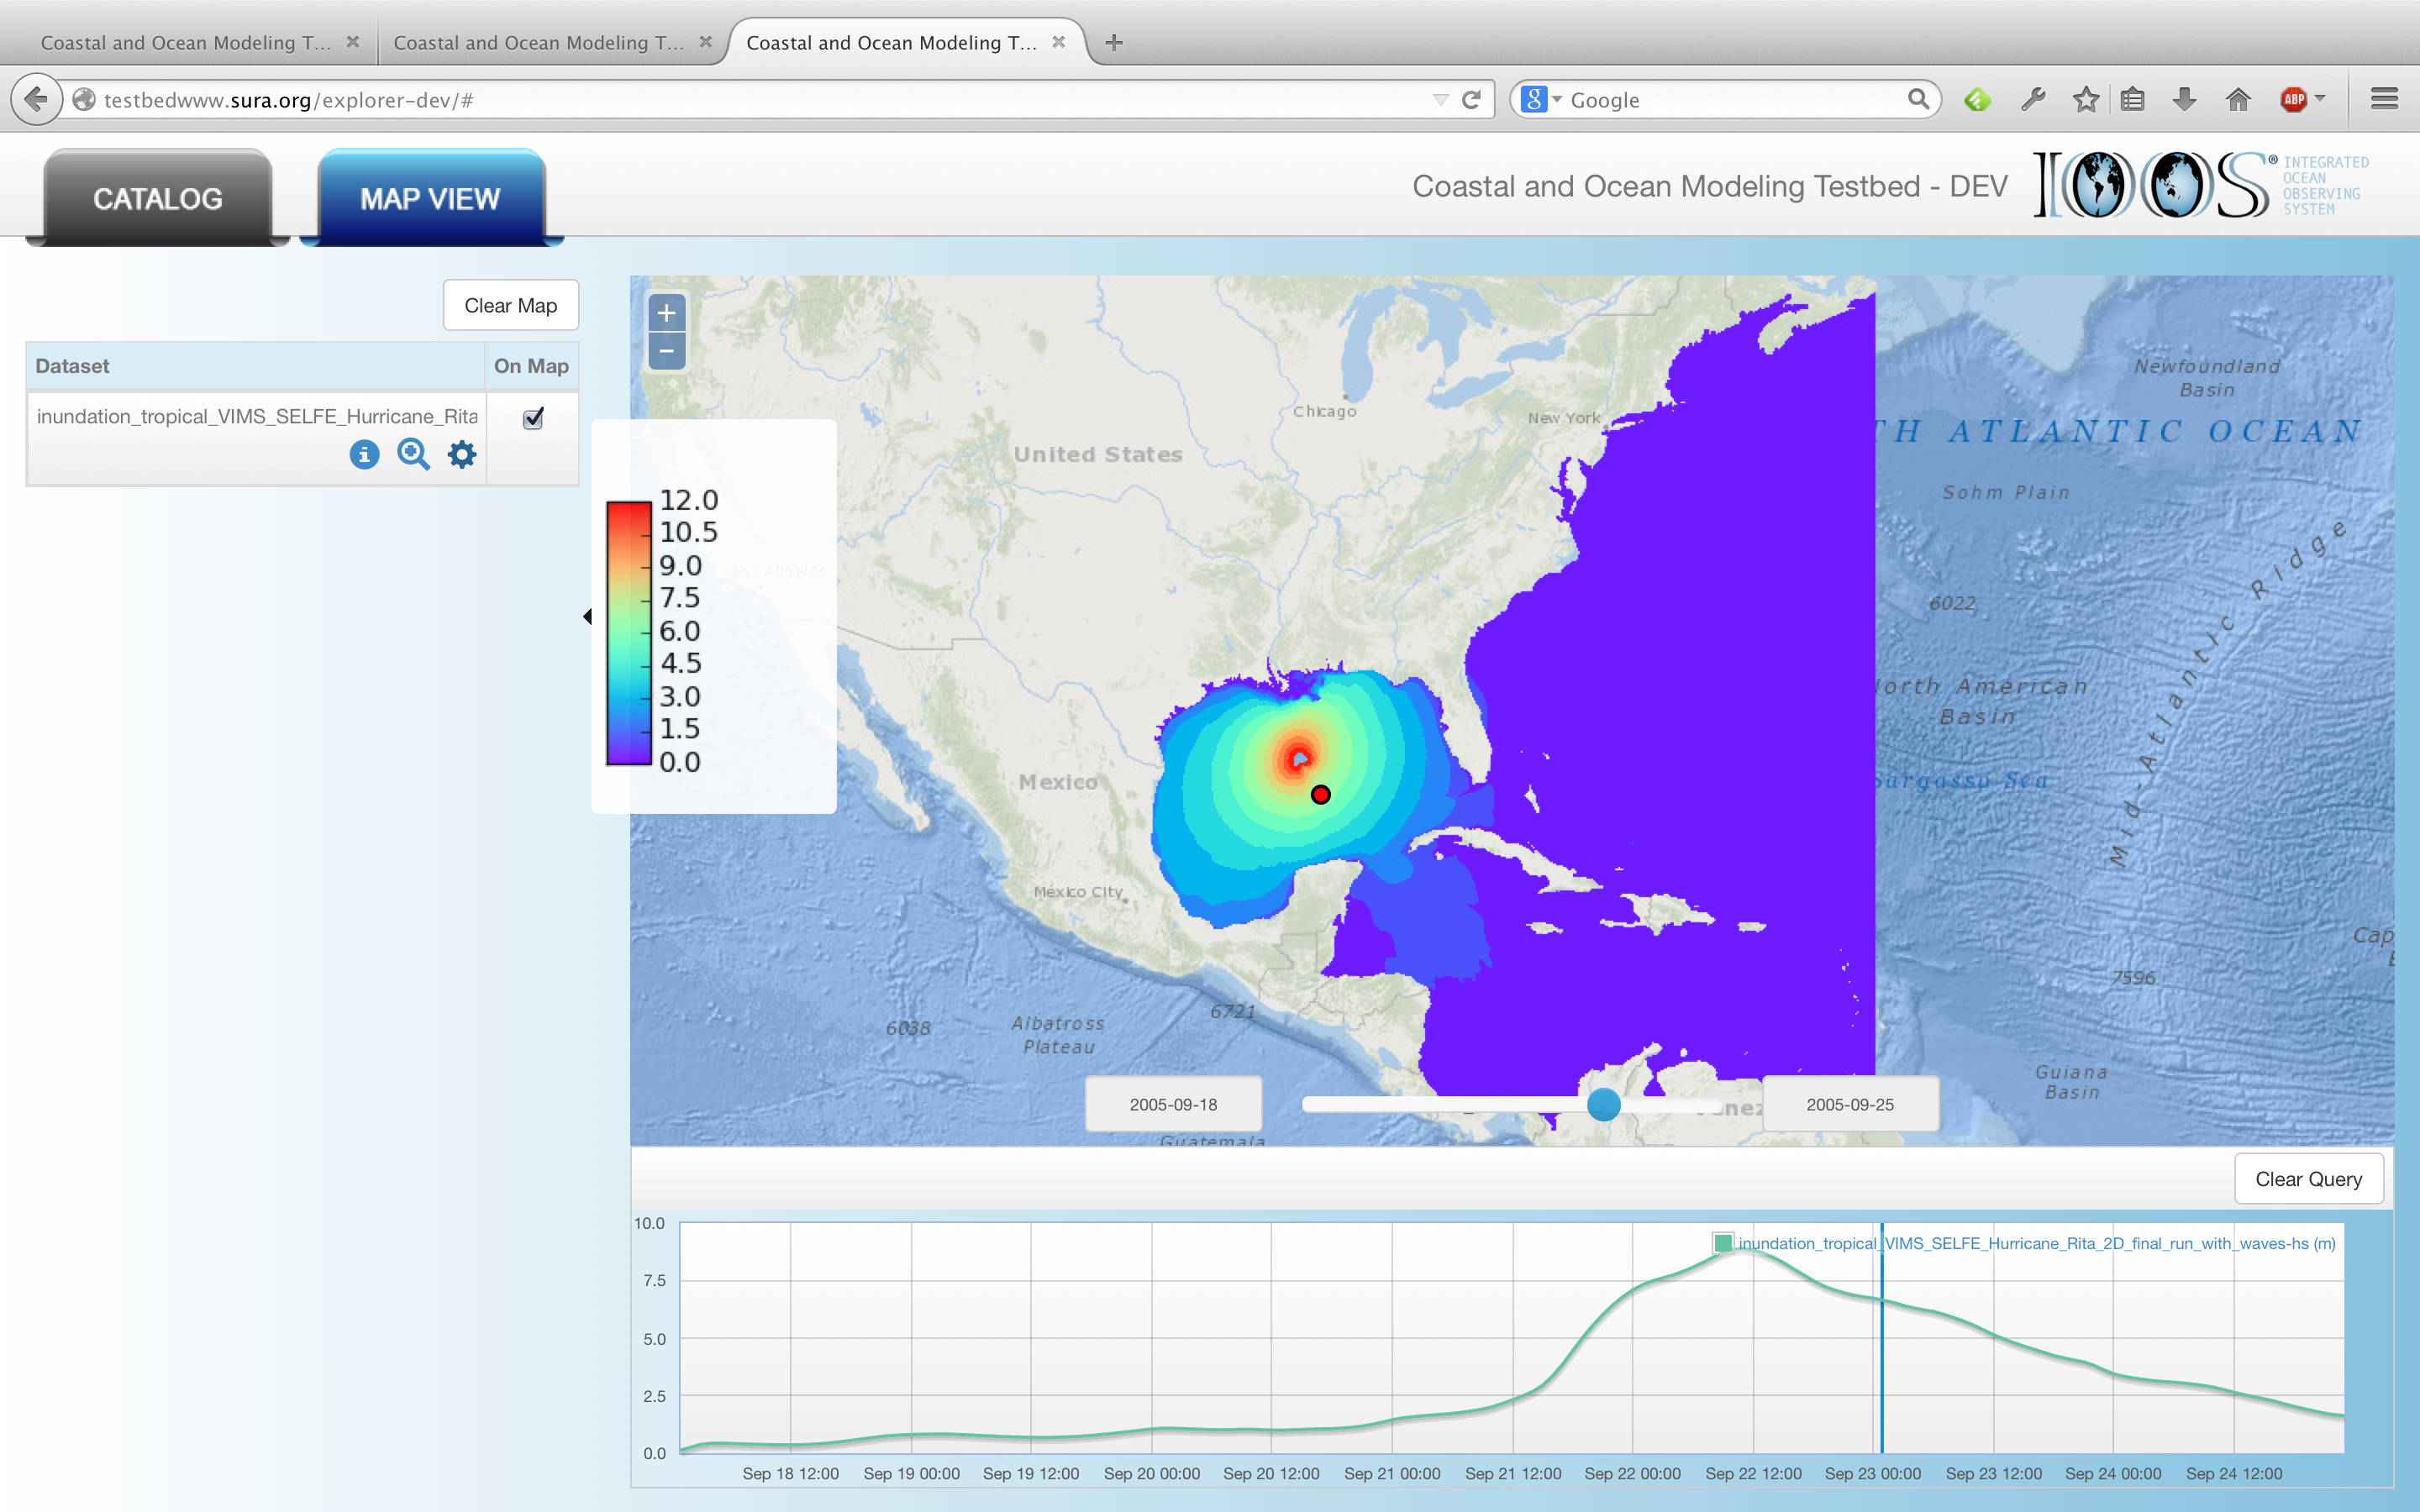
\includegraphics[width=\columnwidth]{../figs/inundation_tropical_VIMS_SELFE_hurricane_rita_2d_final_run_with_waves_sea_surface_wave_significant_height}
    \caption{Visualizing SELFE model of significant sea surface wave height along the eastern coast of the United States. The underlying topology is an unstructured grid with over 5 million nodes which SCI-WMS can handle in real time.}
  \end{subfigure}
\end{figure}


%% \begin{figure}[ht!]
%%   \centering
%%   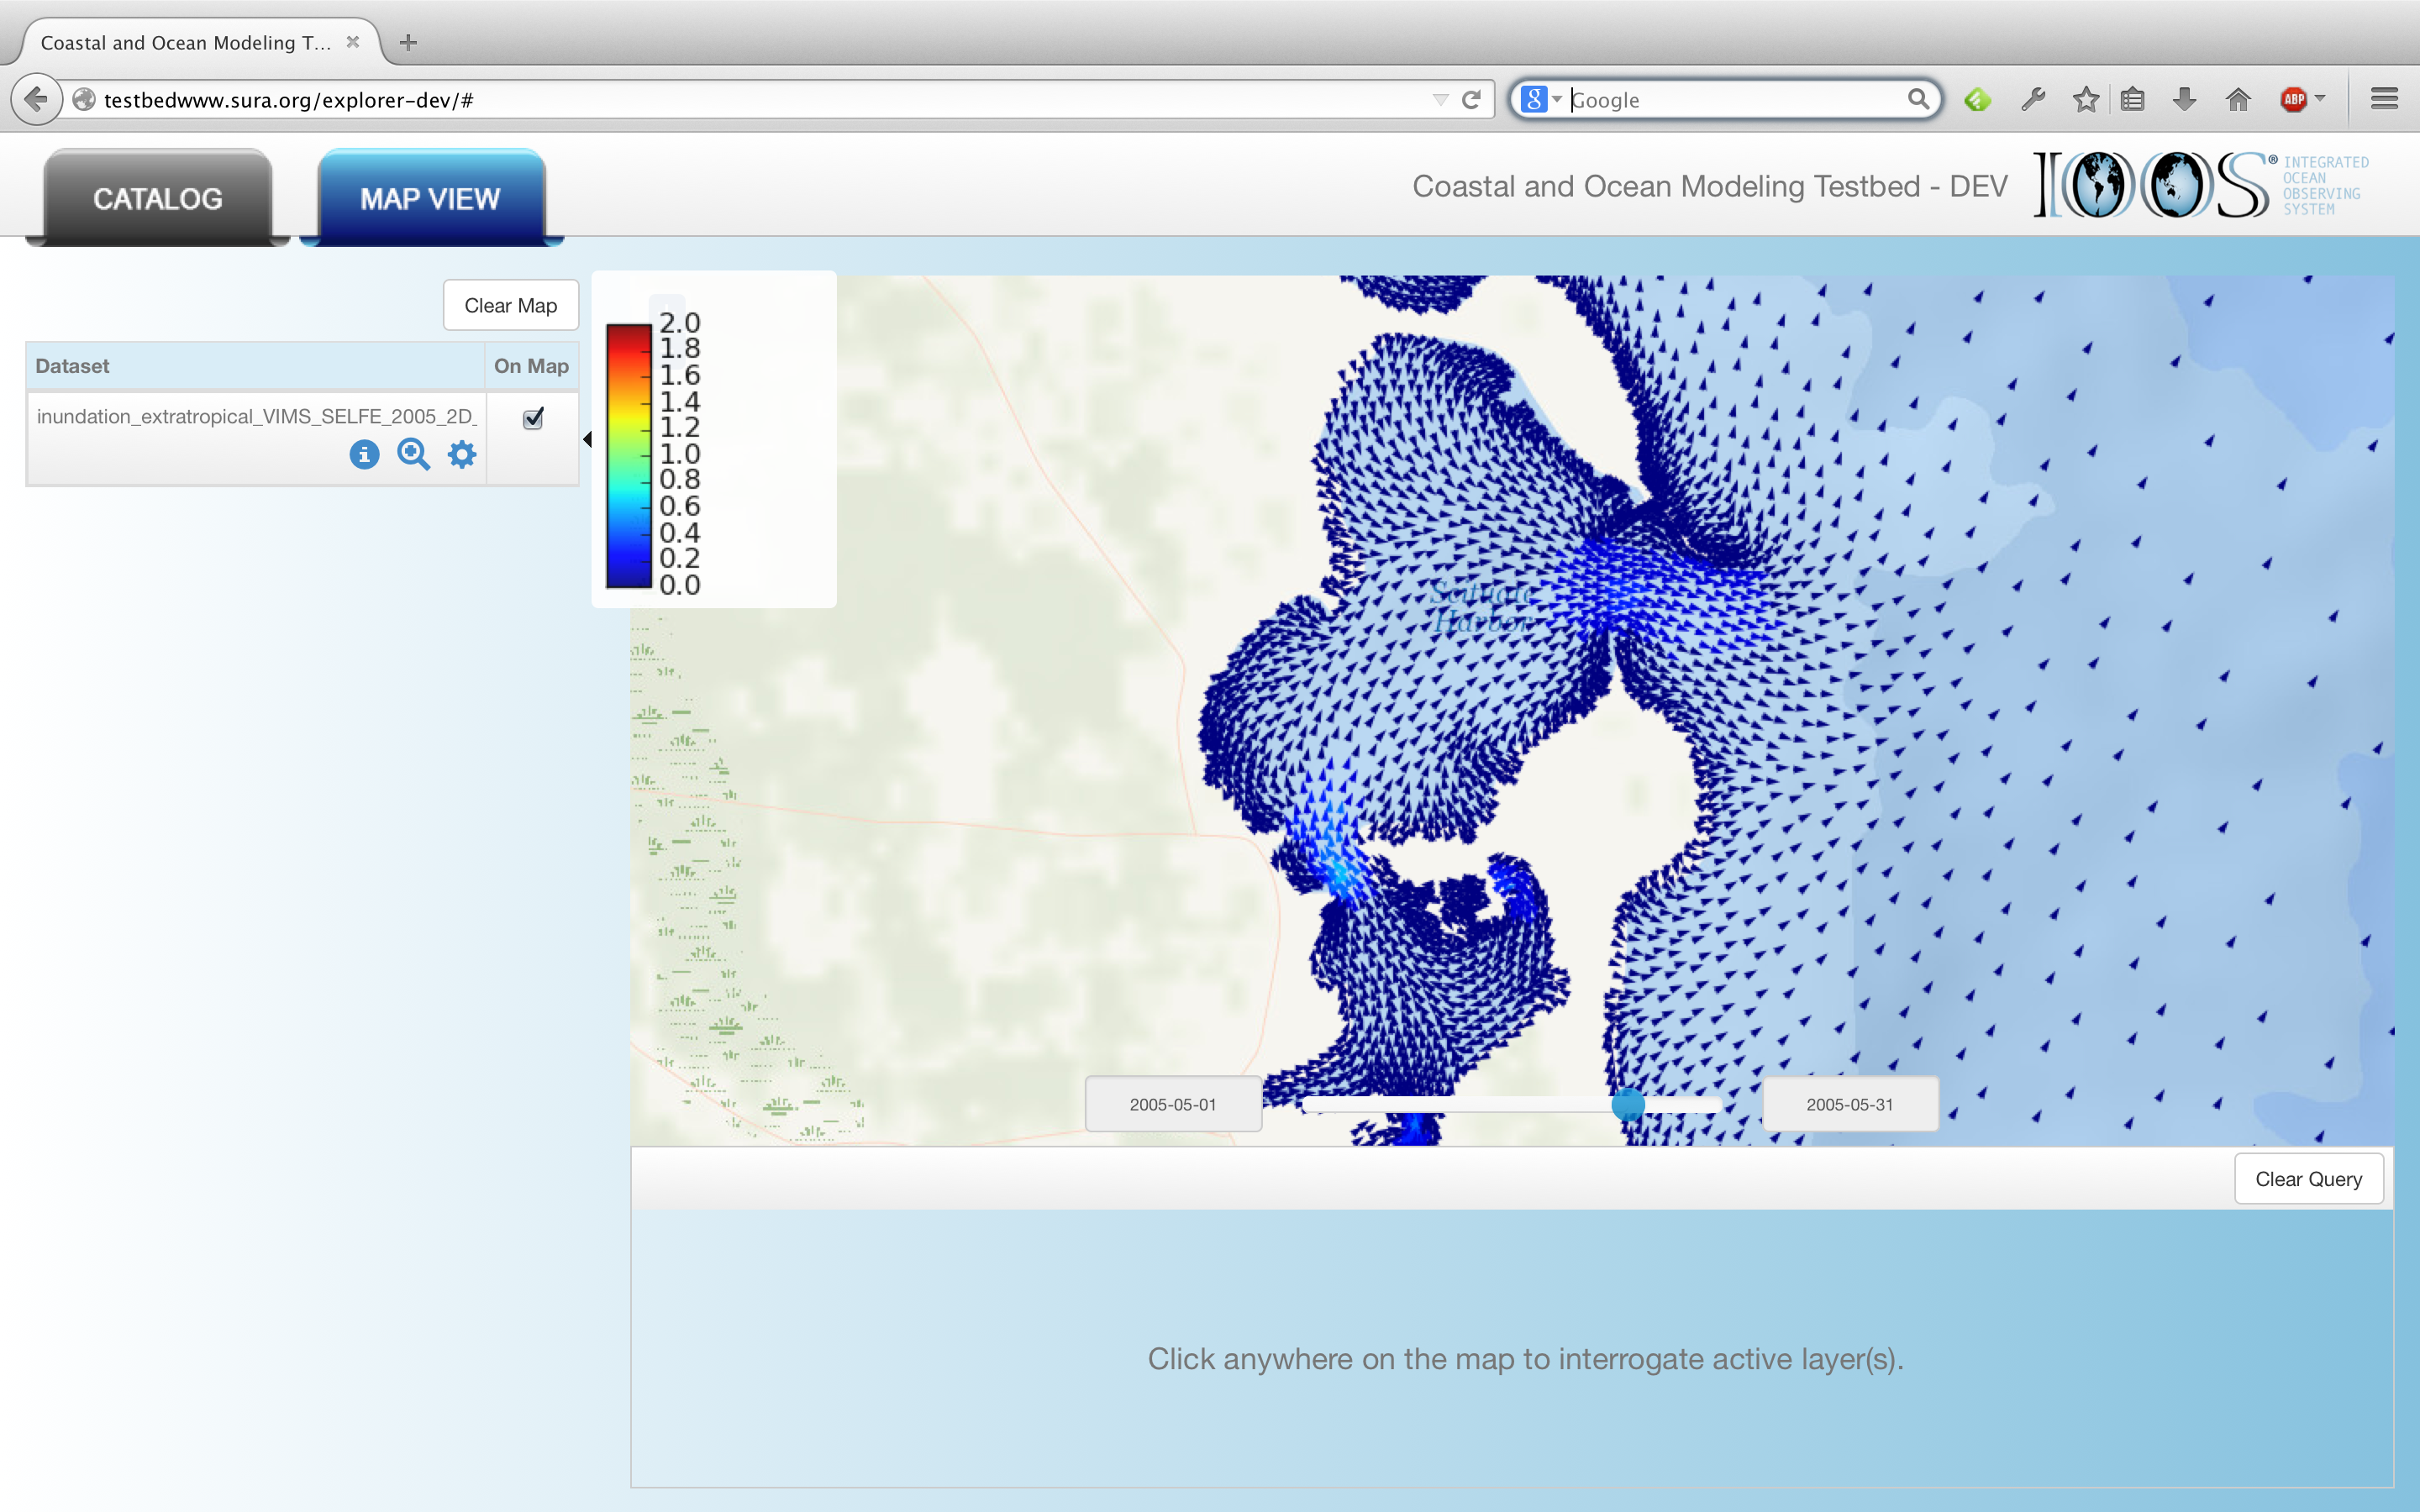
\includegraphics[width=\columnwidth]{../figs/vims_selfe_ubaratropic_vbaratropic_chesapeake_bay}
%%     \caption{SELFE model of current
%%     direction and speed in the Chesapeake Bay area.}
%% \end{figure}

%% \begin{figure}[ht!]
%%   \centering
%%   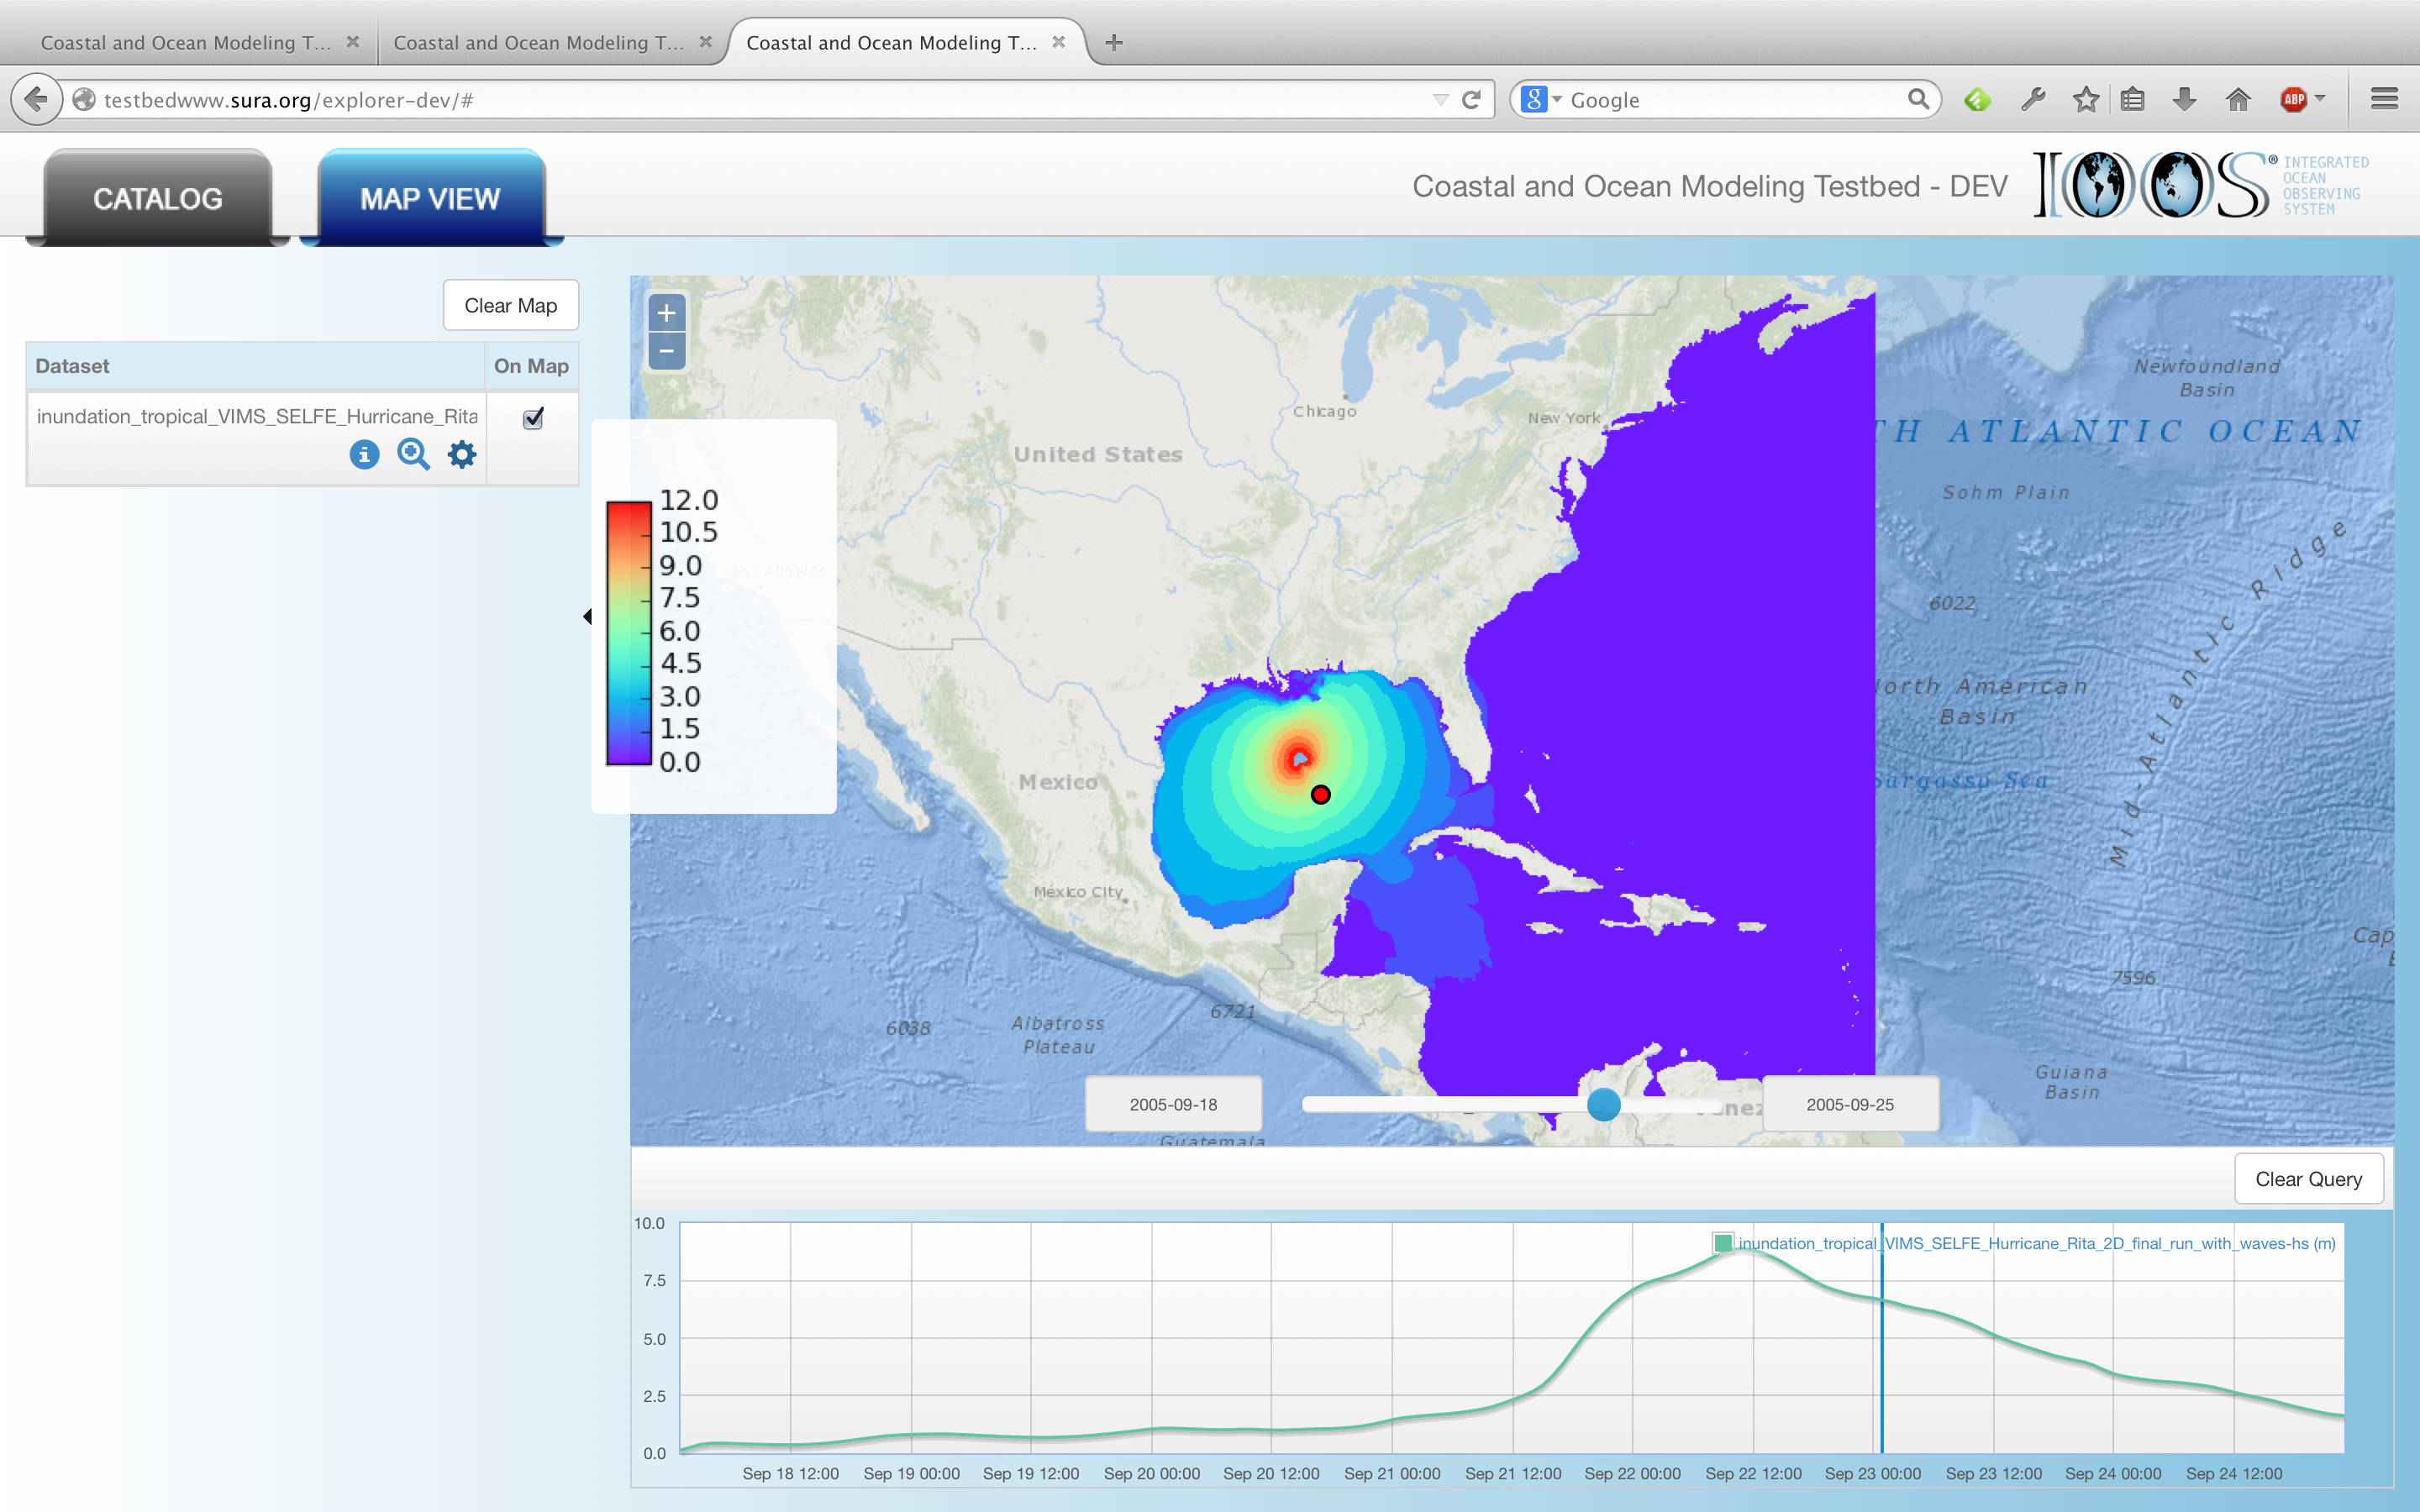
\includegraphics[width=\columnwidth]{../figs/inundation_tropical_VIMS_SELFE_hurricane_rita_2d_final_run_with_waves_sea_surface_wave_significant_height}
%%   \caption{Visualizing SELFE model of significant sea surface wave height along the eastern coast of the United States. The underlying topology is an unstructured grid with over 5 million nodes which SCI-WMS can handle in real time.}
%% \end{figure}
